% Normal forms of vector fields
% We discuss a few theoretical properties of normal forms of vector fields and a
% method for computation. Computing the normal form of a vector field $a(x)$ at a root $x_0$ provides a
% diffeomorphism that maps the stable, unstable, and center manifolds of
% $x_0$ to the eigenspaces of the linearized differential equation
% $\dot{x}=a'(x_0)x$. A method for computation consists of casting a sequence
% of linear transformations to numerical linear algebra.


\documentclass[10pt,T]{beamer}
\usepackage[english]{babel}
\usepackage{graphicx}
\usepackage{amsfonts}
\usepackage{amsmath} % \text{}
\usepackage{amssymb}
\usepackage{amsthm}
\usepackage{enumerate}
\usepackage{libertine}
\usepackage[T1]{fontenc}
\usepackage{tikz-cd}

\tikzset{
	onslide/.code args={<#1>#2}{\only<#1>{\pgfkeysalso{#2}}}
}

% for listing code
\usepackage{listings}
\lstdefinestyle{lststyle}{
	backgroundcolor=\color{white},
	commentstyle=\color{blue},
	keywordstyle=\color{red},
	numberstyle=\tiny\color{black},
	stringstyle=\color{blue},
% 	basicstyle=\small\ttfamily,
        basicstyle=\scriptsize,
	breakatwhitespace=false,
	breaklines=true,
	captionpos=t,
	keepspaces=true,
	numbers=left,                    
	numbersep=5pt,                  
	showspaces=false,                
	showstringspaces=false,
	showtabs=false,                  
	tabsize=3,
	stepnumber=0,
	frame=tb,
	escapeinside={($}{$)}
}
\lstset{style=lststyle}

\renewcommand*\familydefault{\sfdefault}  %% Only if the base font of the document is to be sans serif
\usetikzlibrary{matrix,arrows,decorations.pathmorphing}

\DeclareMathOperator{\tr}{tr}
\DeclareMathOperator{\Diff}{\text{Diff}}

\definecolor{lightgray}{gray}{0.75}
\newcommand{\transparent}[1]{\textcolor{lightgray}{#1}}

%\setbeamerfont{}{shape=\itshape,family=\rmfamily}

%\usepackage[utf8]{inputenc}
%\usepackage{times}
%\usepackage[T1]{fontenc}
%\usepackage[font={footnotesize,it}]{caption}
%\usepackage{natbib}
%\usepackage{multimedia}
%\usepackage{transparent}
%\usepackage{textpos}
%\usepackage{extrabeamercmds}

% ATE
\mode<presentation>
{
\usetheme{Szeged}
\usecolortheme{seagull}
\useinnertheme{circles}
\useoutertheme{default}
\usefonttheme{professionalfonts}
\setbeamercovered{highly dynamic}
}


%\mode<presentation>
%{
%\usetheme{Szeged}
%%\usetheme{Warsaw}
%\usecolortheme{dove}
%\useinnertheme{circles}
%\useoutertheme{default}
%%\usefonttheme{professionalfonts}
%\setbeamercovered{highly dynamic}
%}

%\setbeamersize{⟨options⟩}
%∙ text margin left=⟨TEX dimension⟩ sets a new left margin. This excludes the left sidebar. Thus, it
%is the distance between the right edge of the left sidebar and the left edge of the text.
%∙ text margin right=⟨TEX dimension⟩ sets a new right margin.
%∙ sidebar width left=⟨TEX dimension⟩ sets the size of the left sidebar. Currently, this command
%should be given before a shading is installed for the sidebar canvas.
%∙ sidebar width right=⟨TEX dimension⟩ sets the size of the right sidebar.
%∙ description width=⟨TEX dimension⟩ sets the default width of description labels, see Section 12.1.
%∙ description width of=⟨text⟩ sets the default width of description labels to the width of the ⟨text⟩,
%see Section 12.1.
%∙ mini frame size=⟨TEX dimension⟩ sets the size of mini frames in a navigation bar. When two mini
%frame icons are shown alongside each other, their left end points are ⟨TEX dimension⟩ far apart.
%∙ mini frame offset=⟨TEX dimension⟩ set an additional vertical offset that is added to the mini frame
%size when arranging mini frames vertically
\setbeamersize{text margin left=5mm,text margin right=5mm}

\title[Normal forms of vector fields]{Normal forms of vector fields\\ \small{Python notebook at \texttt{github.com/joepatmckenna/gss}}}
%\subtitle{}

%\centerline{\textbf{\underline{Joseph McKenna$^1$}, \underline{Matthew J. Merrins$^2$}, \underline{Leslie S. Satin$^3$}, \underline{Arthur Sherman$^4$}, \underline{Richard Bertram$^1$}}}
%\centerline{$^1$\emph{Florida State University, 1017 Academic Way, Room 208 Love Building, Tallahassee, FL 32306}}
%\centerline{$^2$\emph{University of Wisconsin-Madison, VA Research (151), Room C3127, 2500 Overlook Terrace, Madison, WI 53705}}
%\centerline{$^3$\emph{University of Michigan School of Medicine, 5128 Brehm Tower, Ann Arbor, Michigan, 48105}}
%\centerline{$^4$\emph{National Institutes of Health, Building 12A, Room 4007, 12 South Dr. MSC 5621, Bethesda, MD, 20892}}
%\centerline{$^1$\emph{tel: 443-995-7788, fax: 850-644-4053, email: jmckenna@fsu.edu}}

\author[McKenna, Joseph P.]{Joseph P. McKenna}
\institute[Florida State University] 
{
  {\small Graduate Student Seminar\\}
}
\date[February 17, 2017]{February 17, 2017}
%\subject{subject}
%\pgfdeclareimage[height=0.7cm]{university-logo}{fig/fsu_seal}
%\logo{\pgfuseimage{university-logo}}

% Table of contents at beginning of each section
\AtBeginSubsection[]
{
  \begin{frame}<beamer>{Outline}
    \tableofcontents[currentsection,currentsubsection]
  \end{frame}
}

\AtBeginSection[]
{
    \begin{frame}<beamer>
    \frametitle{Outline}
    \tableofcontents[currentsection]
    \end{frame}
}

\begin{document}

%\addtocounter{framenumber}{} 
%\setbeamertemplate{footline}[default] 

%
%
% Title and TOC
%
%
\begin{frame}
\titlepage
\end{frame}

\begin{frame}{Outline}
\tableofcontents
\end{frame}

\section{Introduction}

\begin{frame}{Introduction}
\begin{columns}[T,onlytextwidth]	
\column{\textwidth}
\begin{block}{Overview}
\begin{itemize}
\item Goal: Transform the o.d.e. $\dot{x}=f(x)$ near an
  equilibrium $x_0$ to the simplest orbitally equivalent equation.\\[5mm]
\item Method: Perform a sequence of substitutions $x=\psi(\xi)$ that
  zero out terms in the Taylor series of $f(x)$.\\[5mm]
  \item Result: A module describing the `essential' Taylor series terms. A diffeomorphism that maps the
    invariant manifolds of $x_0$ to the eigenspaces of the linearized equation $\dot{x}=f'(x_0)x$.
\end{itemize}
\end{block}
\end{columns}
\end{frame}

\begin{frame}{Substitution}
\begin{columns}[T,onlytextwidth]	
\column{\textwidth}
\begin{itemize}
\item<1-> How does the substitution $x=\psi(\xi)$ transform the o.d.e. $\dot{x}=f(x)$?\\[5mm]
\end{itemize}
\begin{equation*}
\begin{aligned}
\onslide<2->{\psi'(\xi)~\dot{\xi}&=\dot{x}&\text{differentiate }x=\psi(\xi)\\}
\onslide<3->{\dot{\xi}&=\psi'(\xi)^{-1}~\dot{x}&\text{left-multiply by }\psi'(\xi)^{-1}\\}
\onslide<4->{&=\psi'(\xi)^{-1}~f(\psi(\xi))&\text{substitute }\dot{x}=f(x)=f(\psi(\xi))\\}
\onslide<5->{\dot{x}&=(\psi')^{-1}~f\circ\psi(x)&\text{relabel $\xi\leftarrow x$}\\}
\onslide<6->{&\stackrel{\text{def}}{=}\text{S}_{\psi}f(x)&\\}
\end{aligned}
\end{equation*}
\begin{itemize}
\item<6-> By a `similarity' transformation.
\end{itemize}
\end{columns}
\end{frame}

\begin{frame}{Substitution}
\begin{columns}[T,onlytextwidth]	
\column{\textwidth}
\begin{itemize}
\item<1-> How can we calculate $\text{S}_{\psi}f(x)$?
\item<2-> If $g$ generates the flow $\psi$, then the substitution $x=\psi(\xi)$ transforms $\dot{x}=f(x)$ to
\begin{equation*}
\begin{aligned}
\onslide<2->{\dot{x}&=\text{S}_{\psi}f(x)\sim e^{\text{L}_g}f(x)\\[5mm]}
\onslide<3->{&=\left(I+\text{L}_g+\frac12\text{L}_g^2+\frac1{3!}\text{L}_g^3+\cdots\right)\left( f_1 + f_2 + f_3+ \cdots \right)\\[5mm]}
\end{aligned}
\end{equation*}
where L$_{g}f=f'g-g'f$\\
(Murdock, 2003)
\end{itemize}
\end{columns}
\end{frame}

\begin{frame}{Substitution: one degree at a time}
\begin{columns}[T,onlytextwidth]
\column{\textwidth}
\begin{itemize}
\item<1-> If $g_j$ has degree $j$, then the substitution
  $x=\psi_j(\xi)$ leaves the r.h.s. $f(x)$ unchanged up to degree $j-1$:
\begin{equation*}
\begin{aligned}
\dot{x}\sim&(I+\text{L}_{g_j}+\cdots)(f_1+f_2+\cdots+f_{j-1} + f_j+\cdots)\\
\onslide<2->{=&\underbrace{f_1+\cdots+f_{j-1}}_{\text{unchanged}}+\underbrace{f_j+\text{L}_{g_j}f_1}_{h_j=\text{ new deg }j\text{ term}}+\cdots\\}
\end{aligned}
\end{equation*}
\end{itemize}
\begin{itemize}
\item<3-> Which $g_j$ should we choose?
\begin{equation*}
  \begin{aligned}
    \onslide<4->{h_j&=f_j+f'_1g_j-g_j'f_1\\}
    \onslide<5->{&=f_j-\text{L}_{f_1}g_j\\}
    \onslide<6->{\text{L}_{f_1}g_j&=f_j-h_j}
\end{aligned}
\end{equation*}
\end{itemize}
\end{columns}
\end{frame}

\section{The algorithm}

\begin{frame}{The algorithm}
\begin{columns}[T,onlytextwidth]
\column{\textwidth}
\begin{itemize}
\item At the $j^{th}$ step of normalization, $\text{L}_{f_1}g_j=f_j-h_j$\\[5mm]
\begin{enumerate}
\item<2-> find the degree $j$ generator $g_j$:\\[2mm]
  set $h_j$ to projection of $f_j$ onto $\overline{\text{im}~\text{L}_{f_1}}$ and solve $\text{L}_{f_1}g_j=f_j-h_j$\\[5mm]
\item<3-> perform the substitution $x=\psi_{j}(\xi)$ where $g_j$ generates $\psi_j$:\\[2mm]
  $\dot{x}\sim\left(I+\text{L}_{g_j}+\frac12\text{L}^2_{g_j}+\cdots\right)(f_{1}+f_{2}+f_{3}+\cdots)$\\[5mm]
\end{enumerate}
\item<4-> The composed substitution $x=\psi_k\circ\cdots\circ\psi_3\circ\psi_2(\xi)$ modifies $\dot{x}=f(x)$ to $$\dot{x}=f_1(x)+h_2(x)+h_3(x)+\cdots+h_k(x)+\cdots$$
\end{itemize}
\end{columns}
\end{frame}

\section{An example}

\begin{frame}[t]{An example}
\begin{equation*}
  \begin{aligned}
    \dot{x}_1 &= -x_2 -2x_1x_2 -x_1^3 - x_1^2x_2 -x_1x_2^2 \\
    \dot{x}_2 &= x_1 - x_1^2 - 3x_1^3 - x_1^2x_2 - x_2^3
  \end{aligned}
\end{equation*}
\begin{figure}
  \centering
  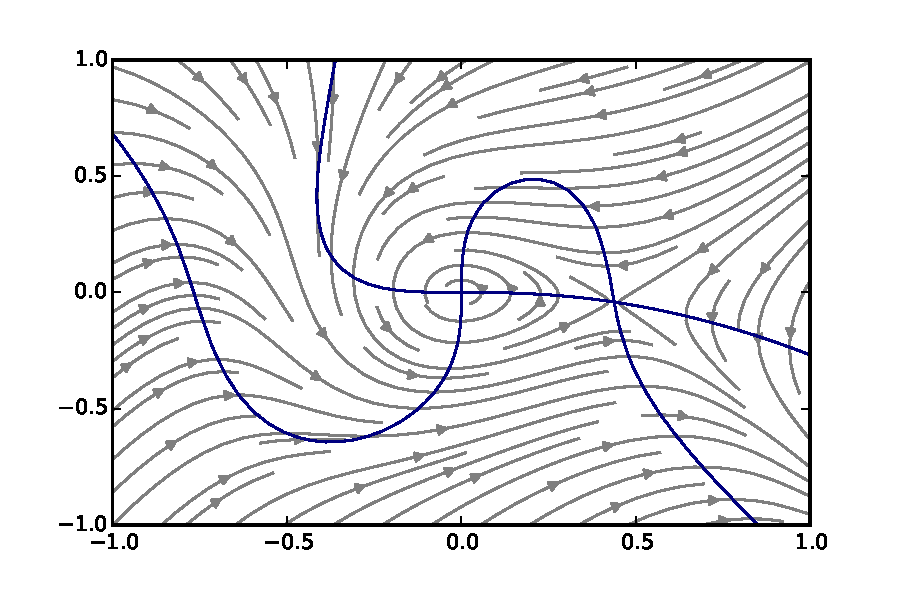
\includegraphics[keepaspectratio,width=.75\textwidth]{./fig/example.pdf}
\end{figure}
\end{frame}

\begin{frame}{An example}
\begin{columns}[T,onlytextwidth]
\column{\textwidth}
\begin{equation*}
  \begin{aligned}
    \onslide<1->{\begin{bmatrix}\dot{x}_1\\\dot{x}_2\end{bmatrix} &= \underbrace{\begin{bmatrix}-x_2\\x_1\end{bmatrix}}_{f_1}+
      \underbrace{\begin{bmatrix}0&-2&0\\-1&0&0\end{bmatrix}\begin{bmatrix}x_1^2\\x_1x_2\\x_2^2\end{bmatrix}}_{f_2}+
      \underbrace{\begin{bmatrix}-1&-1&-1&0\\-3&-1&0&-1\end{bmatrix}\begin{bmatrix}x_1^3\\x_1^2x_2\\x_1x_2^2\\x_2^3\end{bmatrix}}_{f_3}\\[5mm]}
  \onslide<2->{f_1'&=\begin{bmatrix}0&-1\\1&0\end{bmatrix}\\[5mm]}
  \onslide<3->{\text{L}_{f_1}&=[\cdot,f_1]={\Huge ?}}
\end{aligned}
\end{equation*}
\onslide<4->L is (bi)linear, so L$_{f_1}$ must have matrix representation
\end{columns}
\end{frame}

\begin{frame}[b]{Matrix representation of L$_{f_1}$ on $\mathcal{V}_2^2$}
\begin{equation*}
  \onslide<1->{g=\begin{bmatrix}x_1^2\\0\end{bmatrix}}
  \onslide<2->{\Rightarrow\text{L}_{f_1}g=\underbrace{\begin{bmatrix}2x_1&0\\0&0\end{bmatrix}}_{g'}\underbrace{\begin{bmatrix}-x_2\\x_1\end{bmatrix}}_{f_1}
    -\underbrace{\begin{bmatrix}0&-1\\1&0\end{bmatrix}}_{f_1'}\underbrace{\begin{bmatrix}x_1^2\\0\end{bmatrix}}_{g}=\begin{bmatrix}-2x_1x_2\\-x_1^2\end{bmatrix}}
\end{equation*}
\begin{equation*}
  \begin{array}{ccc|ccc|cc}
    \begin{bmatrix}x_1^2\\0\end{bmatrix}&\begin{bmatrix}x_1x_2\\0\end{bmatrix}&\begin{bmatrix}x_2^2\\0\end{bmatrix}&\begin{bmatrix}0\\x_1^2\end{bmatrix}&\begin{bmatrix}0\\x_1x_2\end{bmatrix}&\begin{bmatrix}0\\x_2^2\end{bmatrix}&&\\
    \downarrow&\downarrow&\downarrow&\downarrow&\downarrow&\downarrow&&\\\hline
    \onslide<3->{0}&\transparent{?}&\transparent{?}&\transparent{?}&\transparent{?}&\transparent{?}&\leftarrow&\begin{bmatrix}x_1^2&0\end{bmatrix}^T\\
    \onslide<3->{-2}&\transparent{?}&\transparent{?}&\transparent{?}&\transparent{?}&\transparent{?}&\leftarrow&\begin{bmatrix}x_1x_2&0\end{bmatrix}^T\\
    \onslide<3->{0}&\transparent{?}&\transparent{?}&\transparent{?}&\transparent{?}&\transparent{?}&\leftarrow&\begin{bmatrix}x_2^2&0\end{bmatrix}^T\\\hline
    \onslide<3->{-1}&\transparent{?}&\transparent{?}&\transparent{?}&\transparent{?}&\transparent{?}&\leftarrow&\begin{bmatrix}0&x_1^2\end{bmatrix}^T\\
    \onslide<3->{0}&\transparent{?}&\transparent{?}&\transparent{?}&\transparent{?}&\transparent{?}&\leftarrow&\begin{bmatrix}0&x_1x_2\end{bmatrix}^T\\
    \onslide<3->{0}&\transparent{?}&\transparent{?}&\transparent{?}&\transparent{?}&\transparent{?}&\leftarrow&\begin{bmatrix}0&x_2^2\end{bmatrix}^T
    \end{array}
\end{equation*}
\end{frame}

\begin{frame}[b]{Matrix representation of L$_{f_1}$ on $\mathcal{V}_2^2$}
\begin{equation*}
  \onslide<1->{g=\begin{bmatrix}x_1x_2\\0\end{bmatrix}}
  \onslide<2->{\Rightarrow\text{L}_{f_1}g=\underbrace{\begin{bmatrix}x_2&x_1\\0&0\end{bmatrix}}_{g'}\underbrace{\begin{bmatrix}-x_2\\x_1\end{bmatrix}}_{f_1}
    -\underbrace{\begin{bmatrix}0&-1\\1&0\end{bmatrix}}_{f_1'}\underbrace{\begin{bmatrix}x_1x_2\\0\end{bmatrix}}_{g}=\begin{bmatrix}x_1^2-x_2^2\\-x_1x_2\end{bmatrix}}
\end{equation*}
\begin{equation*}
  \begin{array}{ccc|ccc|cc}
    \begin{bmatrix}x_1^2\\0\end{bmatrix}&\begin{bmatrix}x_1x_2\\0\end{bmatrix}&\begin{bmatrix}x_2^2\\0\end{bmatrix}&\begin{bmatrix}0\\x_1^2\end{bmatrix}&\begin{bmatrix}0\\x_1x_2\end{bmatrix}&\begin{bmatrix}0\\x_2^2\end{bmatrix}&&\\
    \downarrow&\downarrow&\downarrow&\downarrow&\downarrow&\downarrow&&\\\hline
    0&\onslide<3->{1}&\transparent{?}&\transparent{?}&\transparent{?}&\transparent{?}&\leftarrow&\begin{bmatrix}x_1^2&0\end{bmatrix}^T\\
    -2&\onslide<3->{0}&\transparent{?}&\transparent{?}&\transparent{?}&\transparent{?}&\leftarrow&\begin{bmatrix}x_1x_2&0\end{bmatrix}^T\\
    0&\onslide<3->{-1}&\transparent{?}&\transparent{?}&\transparent{?}&\transparent{?}&\leftarrow&\begin{bmatrix}x_2^2&0\end{bmatrix}^T\\\hline
    -1&\onslide<3->{0}&\transparent{?}&\transparent{?}&\transparent{?}&\transparent{?}&\leftarrow&\begin{bmatrix}0&x_1^2\end{bmatrix}^T\\
    0&\onslide<3->{-1}&\transparent{?}&\transparent{?}&\transparent{?}&\transparent{?}&\leftarrow&\begin{bmatrix}0&x_1x_2\end{bmatrix}^T\\
    0&\onslide<3->{0}&\transparent{?}&\transparent{?}&\transparent{?}&\transparent{?}&\leftarrow&\begin{bmatrix}0&x_2^2\end{bmatrix}^T
    \end{array}
\end{equation*}
\end{frame}

\begin{frame}[b]{Matrix representation of L$_{f_1}$ on $\mathcal{V}_2^2$}
\begin{equation*}
  \onslide<1->{g=\begin{bmatrix}x_2^2\\0\end{bmatrix}}
  \onslide<2->{\Rightarrow\text{L}_{f_1}g=\underbrace{\begin{bmatrix}0&2x_2\\0&0\end{bmatrix}}_{g'}\underbrace{\begin{bmatrix}-x_2\\x_1\end{bmatrix}}_{f_1}
    -\underbrace{\begin{bmatrix}0&-1\\1&0\end{bmatrix}}_{f_1'}\underbrace{\begin{bmatrix}x_2^2\\0\end{bmatrix}}_{g}=\begin{bmatrix}2x_1x_2\\-x_2^2\end{bmatrix}}
\end{equation*}
\begin{equation*}
  \begin{array}{ccc|ccc|cc}
    \begin{bmatrix}x_1^2\\0\end{bmatrix}&\begin{bmatrix}x_1x_2\\0\end{bmatrix}&\begin{bmatrix}x_2^2\\0\end{bmatrix}&\begin{bmatrix}0\\x_1^2\end{bmatrix}&\begin{bmatrix}0\\x_1x_2\end{bmatrix}&\begin{bmatrix}0\\x_2^2\end{bmatrix}&&\\
    \downarrow&\downarrow&\downarrow&\downarrow&\downarrow&\downarrow&&\\\hline
    0&1&\onslide<3->{0}&\transparent{?}&\transparent{?}&\transparent{?}&\leftarrow&\begin{bmatrix}x_1^2&0\end{bmatrix}^T\\
    -2&0&\onslide<3->{2}&\transparent{?}&\transparent{?}&\transparent{?}&\leftarrow&\begin{bmatrix}x_1x_2&0\end{bmatrix}^T\\
    0&-1&\onslide<3->{0}&\transparent{?}&\transparent{?}&\transparent{?}&\leftarrow&\begin{bmatrix}x_2^2&0\end{bmatrix}^T\\\hline
    -1&0&\onslide<3->{0}&\transparent{?}&\transparent{?}&\transparent{?}&\leftarrow&\begin{bmatrix}0&x_1^2\end{bmatrix}^T\\
    0&-1&\onslide<3->{0}&\transparent{?}&\transparent{?}&\transparent{?}&\leftarrow&\begin{bmatrix}0&x_1x_2\end{bmatrix}^T\\
    0&0&\onslide<3->{-1}&\transparent{?}&\transparent{?}&\transparent{?}&\leftarrow&\begin{bmatrix}0&x_2^2\end{bmatrix}^T
    \end{array}
\end{equation*}
\end{frame}

\begin{frame}[b]{Matrix representation of L$_{f_1}$ on $\mathcal{V}_2^2$}
\begin{equation*}
  \onslide<1->{g=\begin{bmatrix}0\\x_1^2\end{bmatrix}}
  \onslide<2->{\Rightarrow\text{L}_{f_1}g=\underbrace{\begin{bmatrix}0&0\\2x_1&0\end{bmatrix}}_{g'}\underbrace{\begin{bmatrix}-x_2\\x_1\end{bmatrix}}_{f_1}
    -\underbrace{\begin{bmatrix}0&-1\\1&0\end{bmatrix}}_{f_1'}\underbrace{\begin{bmatrix}0\\x_1^2\end{bmatrix}}_{g}=\begin{bmatrix}x_1^2\\-2x_1x_2\end{bmatrix}}
\end{equation*}
\begin{equation*}
  \begin{array}{ccc|ccc|cc}
    \begin{bmatrix}x_1^2\\0\end{bmatrix}&\begin{bmatrix}x_1x_2\\0\end{bmatrix}&\begin{bmatrix}x_2^2\\0\end{bmatrix}&\begin{bmatrix}0\\x_1^2\end{bmatrix}&\begin{bmatrix}0\\x_1x_2\end{bmatrix}&\begin{bmatrix}0\\x_2^2\end{bmatrix}&&\\
    \downarrow&\downarrow&\downarrow&\downarrow&\downarrow&\downarrow&&\\\hline
    0&1&0&\onslide<3->{1}&\transparent{?}&\transparent{?}&\leftarrow&\begin{bmatrix}x_1^2&0\end{bmatrix}^T\\
    -2&0&2&\onslide<3->{0}&\transparent{?}&\transparent{?}&\leftarrow&\begin{bmatrix}x_1x_2&0\end{bmatrix}^T\\
    0&-1&0&\onslide<3->{0}&\transparent{?}&\transparent{?}&\leftarrow&\begin{bmatrix}x_2^2&0\end{bmatrix}^T\\\hline
    -1&0&0&\onslide<3->{0}&\transparent{?}&\transparent{?}&\leftarrow&\begin{bmatrix}0&x_1^2\end{bmatrix}^T\\
    0&-1&0&\onslide<3->{-2}&\transparent{?}&\transparent{?}&\leftarrow&\begin{bmatrix}0&x_1x_2\end{bmatrix}^T\\
    0&0&-1&\onslide<3->{0}&\transparent{?}&\transparent{?}&\leftarrow&\begin{bmatrix}0&x_2^2\end{bmatrix}^T
    \end{array}
\end{equation*}
\end{frame}

\begin{frame}[b]{Matrix representation of L$_{f_1}$ on $\mathcal{V}_2^2$}
\begin{equation*}
  \onslide<1->{g=\begin{bmatrix}0\\x_1x_2\end{bmatrix}}
  \onslide<2->{\Rightarrow\text{L}_{f_1}g=\underbrace{\begin{bmatrix}0&0\\x_2&x_1\end{bmatrix}}_{g'}\underbrace{\begin{bmatrix}-x_2\\x_1\end{bmatrix}}_{f_1}
    -\underbrace{\begin{bmatrix}0&-1\\1&0\end{bmatrix}}_{f_1'}\underbrace{\begin{bmatrix}0\\x_1x_2\end{bmatrix}}_{g}=\begin{bmatrix}x_1x_2\\x_1^2-x_2^2\end{bmatrix}}
\end{equation*}
\begin{equation*}
  \begin{array}{ccc|ccc|cc}
    \begin{bmatrix}x_1^2\\0\end{bmatrix}&\begin{bmatrix}x_1x_2\\0\end{bmatrix}&\begin{bmatrix}x_2^2\\0\end{bmatrix}&\begin{bmatrix}0\\x_1^2\end{bmatrix}&\begin{bmatrix}0\\x_1x_2\end{bmatrix}&\begin{bmatrix}0\\x_2^2\end{bmatrix}&&\\
    \downarrow&\downarrow&\downarrow&\downarrow&\downarrow&\downarrow&&\\\hline
    0&1&0&1&\onslide<3->{0}&\transparent{?}&\leftarrow&\begin{bmatrix}x_1^2&0\end{bmatrix}^T\\
    -2&0&2&0&\onslide<3->{1}&\transparent{?}&\leftarrow&\begin{bmatrix}x_1x_2&0\end{bmatrix}^T\\
    0&-1&0&0&\onslide<3->{0}&\transparent{?}&\leftarrow&\begin{bmatrix}x_2^2&0\end{bmatrix}^T\\\hline
    -1&0&0&0&\onslide<3->{1}&\transparent{?}&\leftarrow&\begin{bmatrix}0&x_1^2\end{bmatrix}^T\\
    0&-1&0&-2&\onslide<3->{0}&\transparent{?}&\leftarrow&\begin{bmatrix}0&x_1x_2\end{bmatrix}^T\\
    0&0&-1&0&\onslide<3->{-1}&\transparent{?}&\leftarrow&\begin{bmatrix}0&x_2^2\end{bmatrix}^T
    \end{array}
\end{equation*}
\end{frame}

\begin{frame}[b]{Matrix representation of L$_{f_1}$ on $\mathcal{V}_2^2$}
\begin{equation*}
  \onslide<1->{g=\begin{bmatrix}0\\x_2^2\end{bmatrix}}
  \onslide<2->{\Rightarrow\text{L}_{f_1}g=\underbrace{\begin{bmatrix}0&0\\0&2x_2\end{bmatrix}}_{g'}\underbrace{\begin{bmatrix}-x_2\\x_1\end{bmatrix}}_{f_1}
    -\underbrace{\begin{bmatrix}0&-1\\1&0\end{bmatrix}}_{f_1'}\underbrace{\begin{bmatrix}0\\x_2^2\end{bmatrix}}_{g}=\begin{bmatrix}x_2^2\\2x_1x_2\end{bmatrix}}
\end{equation*}
\begin{equation*}
  \begin{array}{ccc|ccc|cc}
    \begin{bmatrix}x_1^2\\0\end{bmatrix}&\begin{bmatrix}x_1x_2\\0\end{bmatrix}&\begin{bmatrix}x_2^2\\0\end{bmatrix}&\begin{bmatrix}0\\x_1^2\end{bmatrix}&\begin{bmatrix}0\\x_1x_2\end{bmatrix}&\begin{bmatrix}0\\x_2^2\end{bmatrix}&&\\
    \downarrow&\downarrow&\downarrow&\downarrow&\downarrow&\downarrow&&\\\hline
    0&1&0&1&0&\onslide<3->{0}&\leftarrow&\begin{bmatrix}x_1^2&0\end{bmatrix}^T\\
    -2&0&2&0&1&\onslide<3->{0}&\leftarrow&\begin{bmatrix}x_1x_2&0\end{bmatrix}^T\\
    0&-1&0&0&0&\onslide<3->{1}&\leftarrow&\begin{bmatrix}x_2^2&0\end{bmatrix}^T\\\hline
    -1&0&0&0&1&\onslide<3->{0}&\leftarrow&\begin{bmatrix}0&x_1^2\end{bmatrix}^T\\
    0&-1&0&-2&0&\onslide<3->{2}&\leftarrow&\begin{bmatrix}0&x_1x_2\end{bmatrix}^T\\
    0&0&-1&0&-1&\onslide<3->{0}&\leftarrow&\begin{bmatrix}0&x_2^2\end{bmatrix}^T
    \end{array}
\end{equation*}
\end{frame}

\begin{frame}{An example}
\begin{columns}[T,onlytextwidth]
\column{\textwidth}
\begin{itemize}
\item ($j=2$) Step 1: Find degree 2 generator $g_2$
\end{itemize}
\begin{equation*}
  \begin{aligned}
    \onslide<1->{\begin{bmatrix}\dot{x}_1\\\dot{x}_2\end{bmatrix} &= \begin{bmatrix}-x_2\\x_1\end{bmatrix}+
      \begin{bmatrix}0&-2&0\\-1&0&0\end{bmatrix}\begin{bmatrix}x_1^2\\x_1x_2\\x_2^2\end{bmatrix}+
     \begin{bmatrix}-1&-1&-1&0\\-3&-1&0&-1\end{bmatrix}\begin{bmatrix}x_1^3\\x_1^2x_2\\x_1x_2^2\\x_2^3\end{bmatrix}\\[5mm]}
    \onslide<2->{&
      \underbrace{\left[\begin{array}{ccc|ccc}
    0&1&&1&&\\
    -2&0&2&&1&\\
    &-1&0&&&1\\\hline
    -1&&&0&1&\\
    &-1&&-2&0&2\\
    &&-1&&-1&0
  \end{array}\right]}_{\text{L}_{f_1}}g_2=\underbrace{\begin{bmatrix}0\\-2\\0\\\hline-1\\0\\0\end{bmatrix}}_{f_2}-h_2}
\onslide<3->{\hspace{5mm}\Rightarrow \left\{\begin{array}{c}h_2=0\\g_2=\begin{bmatrix}x_1^2\\0\end{bmatrix}\end{array}\right.}
\end{aligned}
\end{equation*}
\end{columns}
\end{frame}

\begin{frame}{An example}
\begin{columns}[T,onlytextwidth]
\column{\textwidth}
\begin{itemize}
\item ($j=2$) Step 2: perform substitution $x=\psi_2(\xi)$ where $g_2$ generates $\psi_2$
\end{itemize}
\begin{equation*}
  \begin{aligned}
\onslide<1->{&\begin{bmatrix}\dot{x}_1\\\dot{x}_2\end{bmatrix}\sim\left( I+\text{L}_{g_2}+\frac12\text{L}^2_{g_2}+\cdots \right)(f_1+f_2+f_3+\cdots)\\[5mm]}
    &\begin{array}{cccccccc}
        &\onslide<2->{\text{deg }1}&&\onslide<3->{\text{deg }2}&&\onslide<4->{\text{deg }3}&&\onslide<5->{\text{deg }\geq4}\\\\
        \onslide<2->{=}&\onslide<2->{f_1}&\onslide<3->{+}&\onslide<3->{f_2}&\onslide<4->{+}&\onslide<4->{f_3} &\onslide<5->{+}&\onslide<5->{\cdots}\\
        &&\onslide<3->{+}&\onslide<3->{\text{L}_{g_2}f_1} &\onslide<4->{+}& \onslide<4->{\text{L}_{g_2}f_2} &\onslide<5->{+}& \onslide<5->{\cdots}\\
        &&&&\onslide<4->{+}& \onslide<4->{\frac12\text{L}_{g_2}^2f_1} &\onslide<5->{+}& \onslide<5->{\cdots}\\ 
       \onslide<6->{=} & \onslide<6->{\begin{bmatrix}-x_2\\x_1\end{bmatrix}} & & & \onslide<7->{+}&\onslide<7->{\begin{bmatrix}-1&0&-1&0\\0&-1&0&-1\end{bmatrix}\begin{bmatrix}x_1^3\\x_1^2x_2\\x_1x_2^2\\x_2^3\end{bmatrix}} & \onslide<8->{+} & \onslide<8->{\cdots}
     \end{array}
  \end{aligned}
\end{equation*}
\end{columns}
\end{frame}

\begin{frame}{Matrix representation of L$_{f_1}$ on $\mathcal{V}_3^2$}
\begin{columns}[T,onlytextwidth]
\column{\textwidth}
\begin{equation*}
    \left.\text{L}_{f_1}\right|_{\mathcal{V}_3^2} =
      \left[\begin{array}{cccc|cccc}
               0&1&& & 1&&&\\
               -3&0&2& & &1&&\\
               &-2&0&3 & &&1&\\
               &&-1&0 & &&&1\\\hline
               -1&&& & 0&1&&\\
               &-1&& & -3&0&2&\\
               &&-1& & &-2&0&3\\
               &&&-1 & &&-1&0
      \end{array}\right]
\end{equation*}
\begin{itemize}
\item<2-> $\text{dim}(\ker\left.\text{L}_{f_1}\right|_{\mathcal{V}_3^2})=2$
\item<3-> basis for $\overline{\left.\text{im}~\text{L}_{f_1}\right|_{\mathcal{V}_3^2}}$:
\end{itemize}
\begin{equation*}
\begin{array}{l}
  \onslide<3->{\begin{bmatrix}1&0&1&0&0&1&0&1\end{bmatrix}^T\\}
  \onslide<3->{\begin{bmatrix}0&-1&0&-1&1&0&1&0\end{bmatrix}^T}
\end{array}
\onslide<4->{\Rightarrow h_3 = \alpha_3(x_1^2+x_2^2)\begin{bmatrix}x_1\\x_2\end{bmatrix} + \beta_3(x_1^2+x_2^2)\begin{bmatrix}-x_2\\x_1\end{bmatrix}}
\end{equation*}
\end{columns}
\end{frame}

\begin{frame}{An example}
\begin{columns}[T,onlytextwidth]
\column{\textwidth}
\begin{itemize}
\item ($j=3$) Step 1: Find degree 3 generator $g_3$
\end{itemize}
\begin{equation*}
  \begin{aligned}
    \onslide<1->{\begin{bmatrix}\dot{x}_1\\\dot{x}_2\end{bmatrix} &= \begin{bmatrix}-x_2\\x_1\end{bmatrix}+
      \begin{bmatrix}-1&0&-1&0\\0&-1&0&-1\end{bmatrix}\begin{bmatrix}x_1^3\\x_1^2x_2\\x_1x_2^2\\x_2^3\end{bmatrix}+\cdots\\[5mm]}
    \onslide<2->{&
      \underbrace{\left[\begin{array}{cccc|cccc}
               0&1&& & 1&&&\\
               -3&0&2& & &1&&\\
               &-2&0&3 & &&1&\\
               &&-1&0 & &&&1\\\hline
               -1&&& & 0&1&&\\
               &-1&& & -3&0&2&\\
               &&-1& & &-2&0&3\\
               &&&-1 & &&-1&0
  \end{array}\right]}_{\text{L}_{f_1}}g_3=\underbrace{\begin{bmatrix}-1\\0\\-1\\0\\0\\-1\\0\\-1\end{bmatrix}}_{f_3}-h_3}
\onslide<3->{\Rightarrow \left\{\begin{array}{c}h_3=f_3\\g_3=0\end{array}\right.}
\end{aligned}
\end{equation*}
\end{columns}
\end{frame}

\begin{frame}{An example}
\begin{columns}[T,onlytextwidth]
\column{\textwidth}
\begin{itemize}
\item ($j=3$) Step 2: perform substitution $x=\psi_3(\xi)$ where $g_3$ generates $\psi_3$
\end{itemize}
\begin{equation*}
  \begin{aligned}
\onslide<1->{&\begin{bmatrix}\dot{x}_1\\\dot{x}_2\end{bmatrix}\sim\left( I+\text{L}_{g_3}+\cdots \right)(f_1+h_2+f_3+\cdots)\\[5mm]}
    &\begin{array}{cccccccc}
        &\onslide<2->{\text{deg }1}&&\onslide<3->{\text{deg }2}&&\onslide<4->{\text{deg }3}&&\onslide<5->{\text{deg }\geq4}\\\\
        \onslide<2->{=}&\onslide<2->{f_1}&\onslide<3->{+}&\onslide<3->{f_2}&\onslide<4->{+}&\onslide<4->{f_3} &\onslide<5->{+}&\onslide<5->{\cdots}\\
        &&&&\onslide<4->{+}& \onslide<4->{\text{L}_{g_3}f_1} &\onslide<5->{+}& \onslide<5->{\cdots}\\[5mm]
       \onslide<6->{=} & \onslide<6->{\begin{bmatrix}-x_2\\x_1\end{bmatrix}} & & & \onslide<7->{-}&\onslide<7->{(x_1^2+x_2^2)\begin{bmatrix}x_1\\x_2\end{bmatrix}} & \onslide<8->{+} & \onslide<8->{\cdots}
     \end{array}
  \end{aligned}
\end{equation*}
\end{columns}
\end{frame}

\begin{frame}{An example}
\begin{columns}[T,onlytextwidth]
\column{\textwidth}
\begin{itemize}
\item Normal form truncated at degree 3:
  \begin{equation*}
\begin{bmatrix}\dot{x}_1\\\dot{x}_2\end{bmatrix} = \begin{bmatrix}-x_2\\x_1\end{bmatrix}-\left( x_1^2+x_2^2 \right)\begin{bmatrix}x_1\\x_2\end{bmatrix}
  \end{equation*}
\begin{figure}
  \centering
  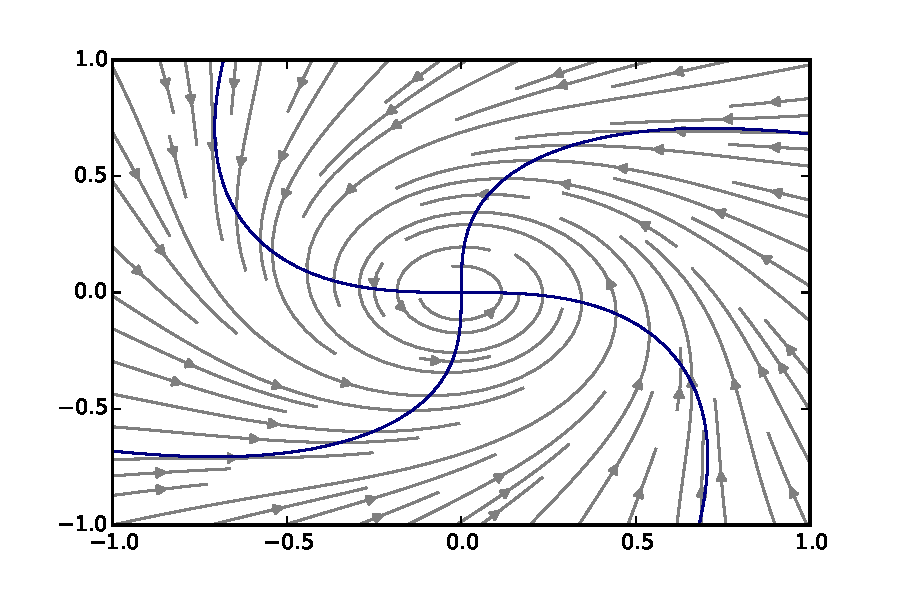
\includegraphics[keepaspectratio,width=.66\textwidth]{./fig/normal.pdf}
\end{figure}
\end{itemize}
\end{columns}
\end{frame}

\begin{frame}{Normal form module}
\begin{columns}[T,onlytextwidth]
\column{\textwidth}
\begin{itemize}
\item<1->
  $\text{dim}(\ker\left.\text{L}_{f_1}\right|_{\mathcal{V}_n^2})
  =\begin{cases}0&n\text{ even}\\2&n\text{ odd}\end{cases}$\\[5mm]
\item<2-> basis for
  $\overline{\left.\text{im}~\text{L}_{f_1}\right|_{\mathcal{V}_n^2}}$ when $n$ odd
  and $m=(n-1)/2$:
\begin{equation*}
  \begin{aligned}
\onslide<2->{&\left[\begin{array}{cccccccccccccc}{m\choose0}&0&{m\choose1}&0&\cdots&{m\choose m}&0 & 0&{m\choose0}&0&{m\choose1}&0&\cdots&{m\choose m}\end{array}\right]^T\\}
\onslide<2->{&\left[\begin{array}{cccccccccccccc}0&-{m\choose0}&0&-{m\choose1}&0&\cdots&-{m\choose m}&{m\choose0}&0&{m\choose1}&0&\cdots&{m\choose m}&0\end{array}\right]^T\\[5mm]}
\onslide<3->{&\Rightarrow h_n = \alpha_n(x_1^2+x_2^2)^m\begin{bmatrix}x_1\\x_2\end{bmatrix} + \beta_n(x_1^2+x_2^2)^m\begin{bmatrix}-x_2\\x_1\end{bmatrix}}
\end{aligned}
\end{equation*}
\item<4-> Normal form module
  \begin{equation*}
\onslide<4->{\ker\text{L}_{f_1}=\mathbb{R}[[r^2]]v_1\oplus\mathbb{R}[[r^2]]v_2}
\end{equation*}
\end{itemize}
\end{columns}
\end{frame}

\begin{frame}{Normal form module}
\begin{columns}[T,onlytextwidth]
\column{\textwidth}
\begin{itemize}
\item<1-> Normal form module
  \begin{equation*}
    \onslide<1->{\ker\text{L}_{f_1}=\mathbb{R}[[(x_1^2+x_2^2)]]\begin{bmatrix}x_1\\x_2\end{bmatrix}\oplus\mathbb{R}[[(x_1^2+x_2^2)]]\begin{bmatrix}-x_2\\x_1\end{bmatrix}}
  \end{equation*}
  \item<2-> $x_1^2+x_2^2$ is a polynomial \emph{invariant} of the flow of
    $f_1=\begin{bmatrix}-x_2\\x_1\end{bmatrix}$
\begin{equation*}
\onslide<2->{\left( \begin{bmatrix}-x_2\\x_1\end{bmatrix}\cdot\nabla \right)(x_1^2+x_2^2) = \begin{bmatrix}-x_2\\x_1\end{bmatrix}\cdot\begin{bmatrix}2x_1\\2x_2\end{bmatrix}=0}
\end{equation*}
\item<3-> $v_1=\begin{bmatrix}x_1\\x_2\end{bmatrix}$ and
  $v_2=\begin{bmatrix}-x_2\\x_1\end{bmatrix}$ are \emph{equivariants} of the flow of $f_1=\begin{bmatrix}-x_2\\x_1\end{bmatrix}$
\begin{equation*}
\onslide<3->{\text{L}_{f_1}v_{i}=0}\onslide<4->{\hspace{5mm}\Rightarrow\text{ the flows of }f_1\text{ and }v_{1},v_2\text{ commute}}
\end{equation*}
\end{itemize}
\end{columns}
\end{frame}

\begin{frame}{Normal form geometry}
\begin{columns}[T,onlytextwidth]
\column{\textwidth}
\begin{itemize}
\item<1-> The flow $\varphi^t$ of the normal form
  $$\dot{x}=\begin{bmatrix}-x_2\\x_1\end{bmatrix}+\sum_{n\geq1}(x_1^2+x_2^2)^n\left(
    \alpha_n\begin{bmatrix}x_1\\x_2\end{bmatrix} +
    \beta_n\begin{bmatrix}-x_2\\x_1\end{bmatrix} \right)$$ preserves the
  foliation $\mathcal{F}$ induced by the linearization flow $\psi=e^{f_1't}$.
\end{itemize}
\onslide<2->{Assume $z_1,z_2$ are on same leaf (circle) of $\mathcal{F}$, so $z_2=\psi(z_1)$.\\}
\onslide<3->{After some time $t$, $\varphi^t(z_2)=\varphi^t(\psi(z_1))=\psi(\varphi^t(z_1))$.\\}
\onslide<4->{Therefore, $\varphi^t(z_1)$, $\varphi^t(z_2)$ are on the same leaf of $\mathcal{F}$.}
\begin{figure}
    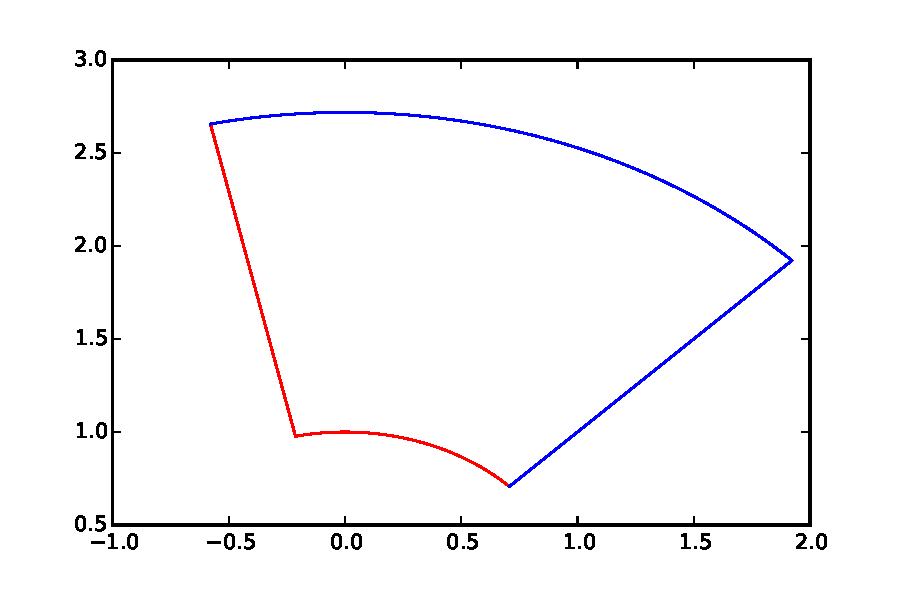
\includegraphics[keepaspectratio,width=.4\textwidth]{./fig/equivariance.pdf}\hspace{3mm}
  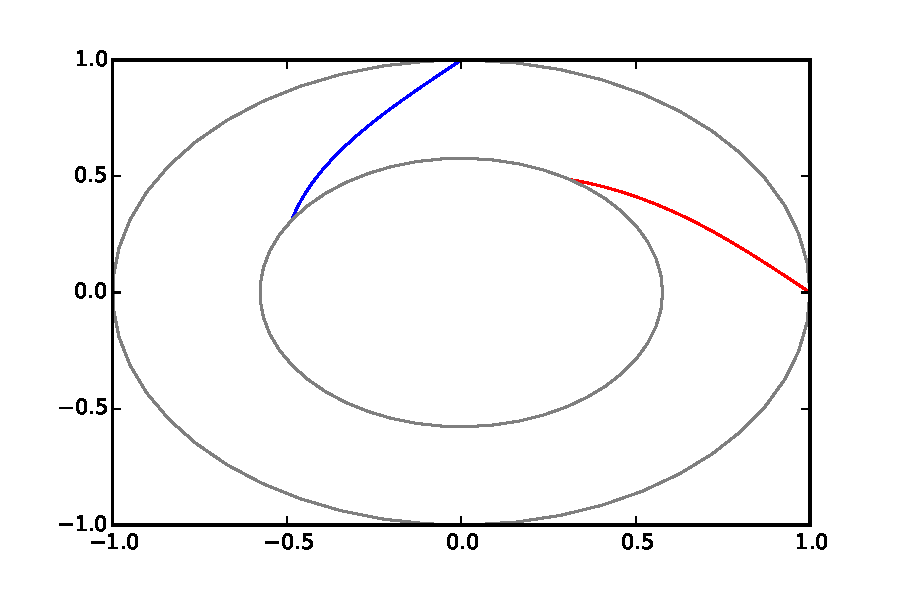
\includegraphics[keepaspectratio,width=.4\textwidth]{./fig/foliation.pdf}
\end{figure}
\end{columns}
\end{frame}

\begin{frame}{The End}
  \begin{center}
    Thanks for coming! Questions?
  \end{center}
\end{frame}

\begin{frame}{Appendix}
\begin{columns}[T,onlytextwidth]	
\column{\textwidth}
\onslide<1->{\begin{theorem}L$_gf=f'g-g'f$\end{theorem}}
\begin{equation*}
\begin{aligned}
\onslide<2->{\frac{d}{ds}\text{S}_{\psi}f&=\frac{d}{ds}(\psi')^{-1}~f\circ\psi&\text{def. of S}_{\psi}\\}
\onslide<3->{&=(\psi')^{-1}~f'\circ\psi~\frac{d}{ds}\psi+\left[\frac{d}{ds}(\psi')^{-1}  \right]~f\circ\psi & \text{prod. \& chain rules}\\}
\onslide<4->{&=(\psi')^{-1}~f'\circ\psi~g\circ\psi-\underbrace{(\psi')^{-1}~g'\circ\psi}_{i.o.u.}~f\circ\psi & g\text{ generates }\psi\\}
\onslide<5->{\frac{d}{ds}\left.\text{S}_{\psi}f\right|_{s=0}&=f'g-g'f&\text{substitute }s=0\\}
\onslide<6->{&\stackrel{\text{def}}{=}\lbrack f,g\rbrack&\text{`Lie bracket'}\\}
\end{aligned}
\end{equation*}
\end{columns}
\end{frame}

\begin{frame}{Appendix}
\begin{columns}[T,onlytextwidth]	
\column{\textwidth}
\onslide<1->{\begin{theorem}S$_{\psi}f=e^{\text{L}_g}f$\end{theorem}}
\begin{equation*}
\begin{aligned}
\onslide<2->{\frac{d}{ds}\text{S}_{\psi}f&=\frac{d}{ds}(\psi')^{-1}f\circ\psi=(\psi')^{-1}~\text{L}_gf\circ\psi&\text{ last slide}\\}
\onslide<3->{\frac{d^j}{ds^j}\text{S}_{\psi}f&=(\psi')^{-1}~\text{L}^j_gf\circ\psi&\text{ iteration}\\}
\onslide<4->{\frac{d^j}{ds^j}\left.\text{S}_{\psi}f\right|_{s=0}&=\text{L}^j_gf&\text{ substitute }s=0\\}
\onslide<5->{\text{S}_{\psi}f&=\left(I+\text{L}_g+\frac1{2!}\text{L}^2_g+\cdots\right)f&\text{ Taylor series}\\}
% \onslide<7->{&=e^{\text{L}_g}f&\\}
\end{aligned}
\end{equation*}
\end{columns}
\end{frame}

\begin{frame}[fragile]{Appendix}
\[
\begin{tikzpicture}[descr/.style={fill=white}]
\matrix(m)[matrix of math nodes, row sep=4em, column sep=5em]
{\psi & \varphi & \transparent{\psi^{-1}\circ\varphi\circ\psi} \\
g & f & (\psi')^{-1}~f\circ\psi\\
& & \lbrack f,g\rbrack \\};
\path[->] (m-1-1) edge node[left] {D$_s$} (m-2-1);
\transparent{\path[->] (m-1-2) edge node[above] {C$_{\psi}$} (m-1-3);}
\path[->] (m-1-2) edge node[left] {D$_t$} (m-2-2);
\transparent{\path[->] (m-1-3) edge node[right] {D$_t$} (m-2-3);}
\path[->] (m-2-2) edge node[above] {S$_{\psi}$} (m-2-3);
\path[->] (m-2-2) edge node[below left] {L$_g$} (m-3-3);
\path[->] (m-2-3) edge node[right] {D$_s$} (m-3-3);
\end{tikzpicture}
\]
\end{frame}

\end{document}
